
\documentclass[11pt]{article}

\usepackage{graphicx, amssymb}
\usepackage[margin=0.8in]{geometry}

\title{\vspace{-2cm}Qualitative study of maps on the 2d torus}

\author{Martin Horvat}

\date{November, 2009}

\begin{document}

\maketitle

A trajectory $\{(x^t,y^t) : t = 0, 1,2,...\}$ of a discrete dynamical system $\phi^t:\mathbb{T}\to\mathbb{T}$ defined over a the two-dimensional torus $\mathbb{T}=[0,L_1]\times[0,L_2]$ is a sequence of points obtained via iteration
%
$$
(x^{t+1},y^{t+1}) = \phi(x^t,y^t)\>,
$$ 
%
which can be explicitly written using two function $f,g:\mathbb{T} \to \mathbb{R}$ as
%
$$
\begin{array}{lll}x^{t+1} = f(x^t,y^t) & {\rm mod}& L_1\cr y^{t+1} = g(x^t,y^t) & {\rm mod}& L_2 \end{array}
$$
%
By taking different initial points an plotting the trajectories we obtain so called phase-portrait that to tells alot about the dynamics of such dynamical system. That can be easily done using the program "sim". The $\phi$ map totally defines the dynamical system and therefore usually we call a dynamical system just simply a map. The program "sim" is intended only for a qualitative study of maps (dynamical system) on the 2d torus. For serious work the author suggests that users write their own code without the graphical user interface (GUI) to speed up calculation and increase resolution of results. Nevertheless the program can be of great help in the preliminary scientific research of maps. 

The content of the package is
%
\begin{itemize}
\item \verb|sim.cpp sim.h| : the source that compiles to "sim"
\item \verb|sim.glade| : information about the graphical interface made in GLADE
\item \verb|sim.cfg| : record of saved maps
\end{itemize}

To compile the program you have to do the following:
%
\begin{itemize}
\item install muParser library
\item run \verb|./confugure|
\item run \verb|make|
\end{itemize}
%
For easier work the author suggests that you  copy all necessary files (sim, sim.glade and sim.cfg) to a separate directory and run the program "sim" there. The program sim.cpp and sim.h was written and may be redistributed under GNU Lesser General Public License (LGPL) version 3 and testing was performed on ubuntu 8.10 (linux OS). But please note that the random generator Mersenne Twister in file MersenneTwister.h is redistributed under BSD license.

A screenshot of playing with the standard (Chirikov) map at kicking strenght K=0.8.

\begin{center}
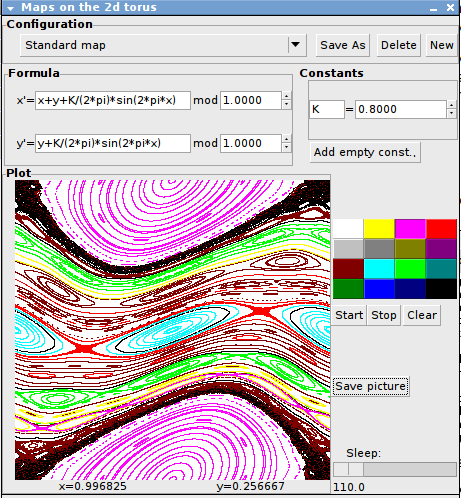
\includegraphics[width=10cm]{screen.png}
\end{center}

The source and the program are in directory \verb|src|. The {\tt muParser} used in the program is \verb|muparser_v130.tar.gz| (in the \verb|src| dir)  or at its the originating site \verb|http://muparser.sourceforge.net|
\end{document}
